 \documentclass[twocolumn,superscriptaddress,aps]{revtex4-1}

\usepackage[utf8]{inputenc}

\usepackage{amsfonts}
\usepackage{amssymb}
\usepackage{amsmath}
\usepackage{amsthm}

\usepackage{bbold}
\usepackage{bm}
\usepackage{graphicx}
\usepackage{color}
\usepackage{hyperref}

\begin{document}


% ==============================================================================

\title{\Large{INFO8010: Project Report}}
\vspace{1cm}
\author{\small{\bf Mathias Beguin}}
\affiliation{\texttt{mathias.beguin@student.uliege.be} (\texttt{s140309})}
\author{\small{\bf Corentin Jemine}}
\affiliation{\texttt{cjemine@student.uliege.be} (\texttt{s123578})}

\maketitle

% ==============================================================================

\section{Abstract}
Despite the many successes of deep learning in the recent years, there remains a disappointment when it comes to the state of the art for source separation in the music domain. This task that appears to be fit for deep learning models intriguingly proves to be challenging and is far from being solved. Most approaches to source separation in audio operate in the time-frequency domain. However, recent deep learning text-to-speech frameworks work directly in the waveform domain. We believe and explore the idea that source separation is also feasible in the waveform domain.


\section{Task definition}
The task is defined as extracting the signal that makes up for a subset of instruments in the waveform of a polyphonic music. Concretely, the model is presented with a single waveform as input that is the combined signal of multiple instruments. The model is expected to output a signal per instrument recognized that corresponds to the signal of that instrument before it was combined.

Several variants exist when it comes to selecting the instruments to extract:
\begin{itemize}
	\item An informed setting, where the model is made aware of instruments present in the musical piece before inference. A typical way of presenting the instruments to the model is through conditioning by either a fixed-size binary vector that corresponds to all instruments seen in training or through a learned embedding in latent space that corresponds to a single instrument (the model is then run several times for each instrument).
	\item A blind setting, where the model has to work out which instruments are present in the musical piece and to extract them.
	\item A fixed setting, where the set of instruments to predict remains constant.
\end{itemize}
Additionally, the model can know how to extract every instrument in the musical piece, or it can only know of a subset of them. In the latter case, it would then be tasked to leave out the remaining instruments together in an "other" target waveform or to simply ignore them.

We operate in a fixed setting. In contrast to \cite{SourceSeparationWaveformDomain}, we allow for musical pieces where some instruments to predict do not appear in the source waveform at all. However, we strictly ensure that instruments that should not be be predicted do also not appear in the source waveform.

\section{Choice of domain}
Most often, audio source separation is performed on a time-frequency representation of the waveform - such as a spectrogram - rather than directly on the waveform, e.g. \cite{DeepConvSep, Tacotron1}. Waveforms make for a much denser representation of audio than spectrograms and are strictly one-dimensional, whereas spectrograms are two-dimensional, allowing to more easily leverage some spatial connectivity. However, the spectrogram is a lossy representation of the audio waveform that discards the phase. Therefore, models that generate a spectrogram of the audio need another generating function to translate the spectrogram into the waveform domain before it becomes playable audio. This transformation is not trivial, however an approximation of the target phase can be obtained from the source phase. This is in contrast with purely generative methods such as text-to-speech, where the waveform has to be generated by a highly non-linear model to obtain a natural sound.

It is becoming increasingly common in deep learning to directly model the target waveform so as to train in an end-to-end fashion, e.g. \cite{Tacotron2, WaveRNN}. In our case, the target signal is fully present in the input signal. Indeed, summing a set of audio waveforms corresponds exactly to a waveform of all signals mixed together, up to a normalizing constant. In light of these facts, we decided to experiment directly in the waveform domain.

\begin{figure*}[t]
	\centering
	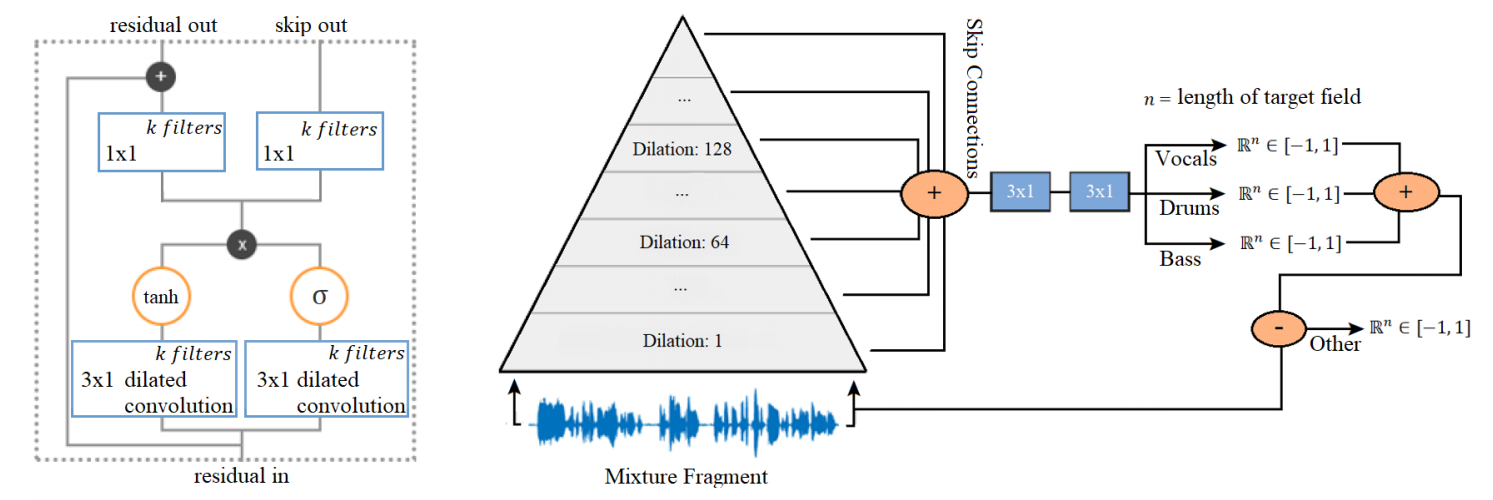
\includegraphics[width=.9\linewidth]{arch.png}
	\caption{The architecture of the Wavenet-based model from \cite{SourceSeparationWaveformDomain}. On the left is a residual block, on the right is a full model with a single stack.}
	\label{arch}
\end{figure*}

\section{Data generation}
Our dataset consists of a large corpus of MIDI files scraped from the web. We generate samples by playing only the requested instruments in each music. Only musics that contain all source instruments are selected. Chunks of $d$ milliseconds of audio are extracted, so as to keep the data batches light in size. Note that only 5 seconds of audio sampled at 44.1kHz already represents 220500 floating-point values. We use heuristics to filter out chunks that would not be effective for training, mainly by ensuring that the source and target waveform differ enough.

Because the data is very dense while MIDI files are fairly small in size, we cannot afford to cache the dataset on the disk. Instead, we build a pool of chunks at runtime and allow chunks to be re-used a second or third time for training. By making the pool large enough and keeping it shuffled, two batches are never identical and a same chunk will usually reappear a few steps after having appeared once. We adjust this chunk reuse factor in function of whether the model training or the data generation is the faster process. Note that with the training being done on the GPU, these two tasks are highly (but not quite embarrassingly) parallel. When $d$ is chosen small, a single piece of music can generate a lot of chunks. In this case, we set the chunk reuse factor to 1 and instead set a fixed limit to how many chunks can be extracted from a piece of music. This allows for more variability in the training data.

\section{Choice of the loss}
We revolve our tests around the choice of the loss. To this end, we consider several loss functions.

A common choice is either the MAE or MSE between each the generated and ground truth waveforms of each target instrument.

We also elaborate a spectrogram-based loss. We can keep the model operating in the waveform domain and still compare the spectrogram of the generated output with the ground truth as a loss. Indeed, the short-time Fourier transform used to derive a spectrogram from an audio waveform is a differentiable operation and can therefore be used in the computation of a loss. It is integrated as a primitive in both Tensorflow and PyTorch. We take the L2 loss between the linear spectrogram of the generated waveform and that of the target waveform for this loss function.

We have experimented with the difference loss $\mathcal{L}_{\text{diff}}$ from~\cite{SourceSeparationWaveformDomain}. It consists in building a matrix $a = n\times n$ where $a_{ij} = |\hat{y}_i - y_j|$. Minimizing the sum of the diagonal of $a$ is equivalent to minimizing the MAE, while maximizing the non-diagonal elements is equivalent to minimizing $\mathcal{L}_{\text{diff}}$ (note that this is a strictly negative loss).

\section{Experiments}
Our baseline model is a simple 4-layer convolutional network with large one-dimensional kernels and ReLU activations. Padding is adjusted to keep the waveform length intact throughout the forward pass. We found this lightweight model to already be performing well on the simpler task of separating a single instrument target from a source composed of multiple instruments. The model performs even better when inserting a skip connection between each two convolutions by summing the output of the convolution with its input. However, the model fails to do well on our task regardless of the selected loss, and typically converges to outputting a constant zero output for all instruments.

We experimented with the Wave-U-Net model from \cite{Wave-U-Net}. Unfortunately, our implementation fails to be better than our baseline. However, our reproduction of the WaveNet-based model from \cite{SourceSeparationWaveformDomain} does perform well. We use this model for the rest of our experiments.

The Wavenet-based model consists of a sequence of stacks that each are made of a sequence of blocks. The model architecture is depicted in figure \ref{arch}. Each block's dilation rate increases exponentially with regard to its position in the stack. This allows to increase the receptive field in a supralinear fashion with respect to the number of layers, as is done in Wavenet \cite{WaveNet}. Blocks produce a residual output that is forwarded in subsequent blocks, and a skip output that is eventually summed with all other skip outputs of the model. The skip outputs are then passed through two convolutional layers (without dilation) and an additional convolutional layer (not shown in figure \ref{arch}) to obtain one waveform per instrument to predict. Chaining stacks is mostly intended to increase the complexity of the model. Note that there is a ReLU activation present after each convolution. Because the instruments to be predicted as target waveform are all present in the source waveform, we do not generate a waveform for unknown instruments at the output of the model.

In our implementation, we use 4 stacks of 10 blocks each. We set the number of filters k to 128, and the number of filters for the final two convolutions to 512 and 256 respectively. These choices are made mostly depending on the available GPU memory at our disposal. Additionally, we find that small chunk durations can suffice as data. The duration should not be too short however, so as to keep blocks with a large dilation factor useful. Following the choice made in \cite{SourceSeparationWaveformDomain}, we set the chunk length $d$ to 100ms, corresponding to 4410 samples per chunk when using 44.1kHz audio. We set the batch size to 12 and use Adam as optimizer with a fixed learning rate of $1\times10^{-4}$. After an analysis of the distribution of instruments in our datasets, we select a set of 10 instruments that should be suitable for prediction. From this set of 10 we select 4 for our experiments: the drums, the piano, a string ensemble and the bass.

We train our model for 1500 steps. We find that the loss does not decrease beyond that. Because we never made a full epoch of the dataset on our trainings, we do not need to check our loss against a validation set. We do however compare the models on a test set. We consider the same model trained with four different losses: the MSE, the MAE, a combination of the spectrogram loss with the MAE and a combination of the difference loss $\mathcal{L}_{\text{diff}}$ with the MAE.

We display our results in table \ref{results}. The MSE and MAE losses tie on most metrics with the exception of the spectrogram error, where the MSE is more destructive than the MAE. The spectrogram loss appears to be more destructive towards the other metrics. The ideal way to evaluate these models would be a mean opinion score rated by several participants. We lack the means to proceed with such an evaluation. We informally find the outputs generated by the model trained with MAE to be slightly more pleasant. 
 
\begin{table}[!h]
	\centering
	\small{%
	\begin{tabular}{c|c|c|c|c}
		&\multicolumn{4}{c}{Evalution metric} \\
		Training loss & MSE & MAE & Spec & $\mathcal{L}_{\text{diff}}$  \\ \hline
		MSE & $3.08\times10^{-2}$ & $\bm{3.5\times10^{-3}}$ & 148.1 & $\bm{-11.6\times10^{-2}}$\\ 
		MAE & $\bm{2.88\times10^{-2}}$ & $4.0\times10^{-3}$ & 85.4 & $-10.9\times10^{-2}$\\ 
		MAE + 0.002Spec & $5.41\times10^{-2}$ & $13.5\times10^{-3}$ & \textbf{67.0} & $-8.2\times10^{-2}$ \\ 
		MAE + $0.2\mathcal{L}_{\text{diff}}$ & $3.61\times10^{-2}$ & $5.6\times10^{-3}$ & 142.6 & $-10.8\times10^{-2}$ \\ 
	\end{tabular}}
	\caption{Training loss vs performance on each evaluation metric. $\mathcal{L}_{\text{diff}}$ is negative, and the lower (highest in absolute value) is better.}
	\label{results}
\end{table}	


\section{Generation}
Because the model occupies a large space in memory, we can only generate the output of an entire music through several passes of small sequential chunks from the input waveform. We cut a fixed-size portion of the audio at the beginning and at the end of each chunk, as zero-padding and convolutions cause artifacts on the edges. We merge the chunks with cross-fading to obtain the full output waveforms. Samples are available here\footnote{\url{https://github.com/CorentinJ/SourceSeparation/blob/master/samples.md}}.

\section{Conclusion}
We find that it is possible to separate instruments on synthesized music with a deep learning model directly operating in the waveform domain. We believe that better results can be obtain through the elaboration of a better loss function.

% ==============================================================================

\bibliographystyle{unsrt}
\bibliography{references}

\end{document}